\chapter{Results}

In this chapter, we present the results for various models on three datasets.\todo{What datasets? Describe or make a reference.} We compare the performance of the models and the datasets. This also includes comparison of open source data downloaded from the Internet with the proprietary data provided by the private company.\todo{What else? There should probably be more.}

\section{Comparison of Models}

In the following text, comparison of the models is presented. We show the accuracy, precision and recall of these models on three datasets.\todo{What models? Explain or provide reference.}\todo{Explanation of these measurement metrics should be somewhere and perhaps a reference would be in order.} This comparison allows us to conclude what model is best for this application.

\subsection{Firefox Data}

On Figure~\ref{fig:results.models.firefox}, you can see the performance of the chosen models on Firefox data. The SVM model with TF-IDF weighing achieves the best performance with accuracy of 57\%. It's precision and recall also outperforms all the other approaches with values of 51\% and 45\%. The same model with LSI takes second place. The only model other than SVM that approaches SVM with it's performance is CART, especially with TF-IDF weighing.

\begin{figure}[htbp]
    \centering
        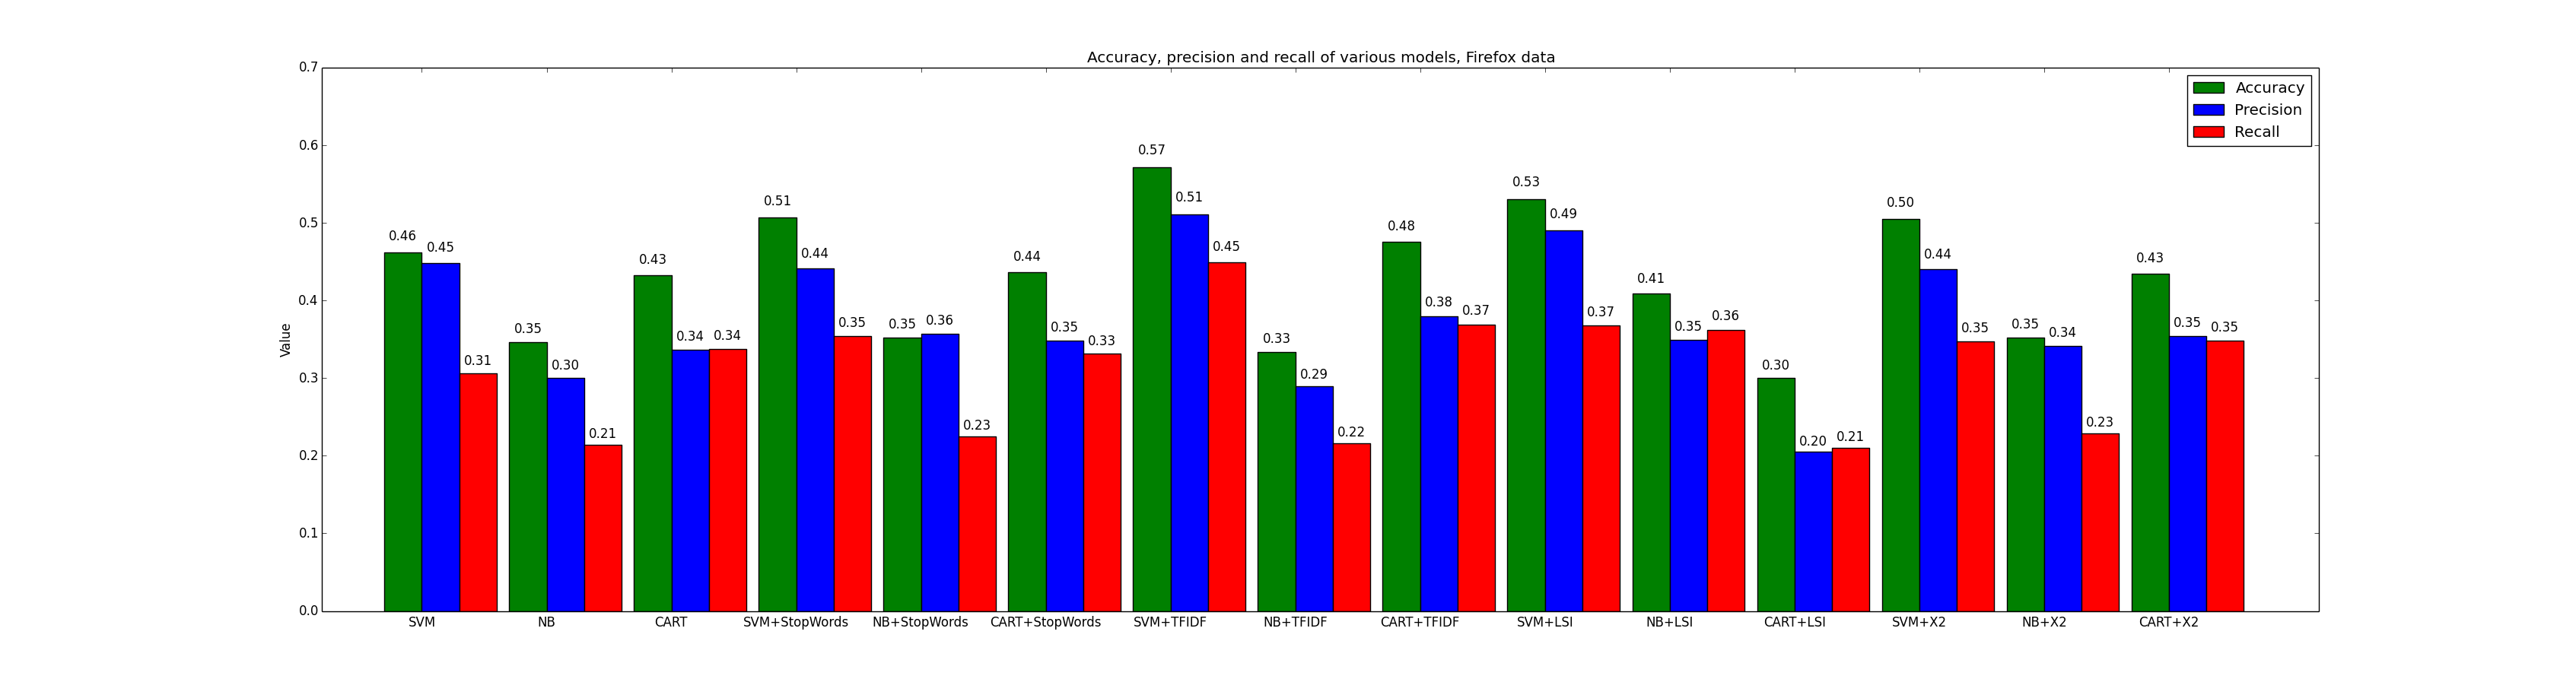
\includegraphics[width=\textwidth,trim=8cm 1cm 8cm 1cm,clip]{./images/comparison_of_models/firefox.png}
    \caption{Comparison of models on Firefox data.}
    \label{fig:results.models.firefox}
\end{figure}

\subsection{Netbeans Data}

The performance of the models on Netbeans data is shown on Figure~\ref{fig:results.models.netbeans}. It is clear that the SVM model with TF-IDF weighing performs best even on the Netbeans data, although in this case the LSI feature extraction technique does not seem to perform as well as in the previous case. The accuracy, precision and recall of the approach are 53\%, 53\% and 49\% respectively. Sole SVM model and SVM+$\chi^2$ model perform similarly as far as precision is concerned, while the accuracy and recall values are lagging behind by a considerable margin. None of the other models offer better performance than even sole SVM model on this data, which suggests that SVM is a very good choice in this domain.

\begin{figure}[htbp]
    \centering
        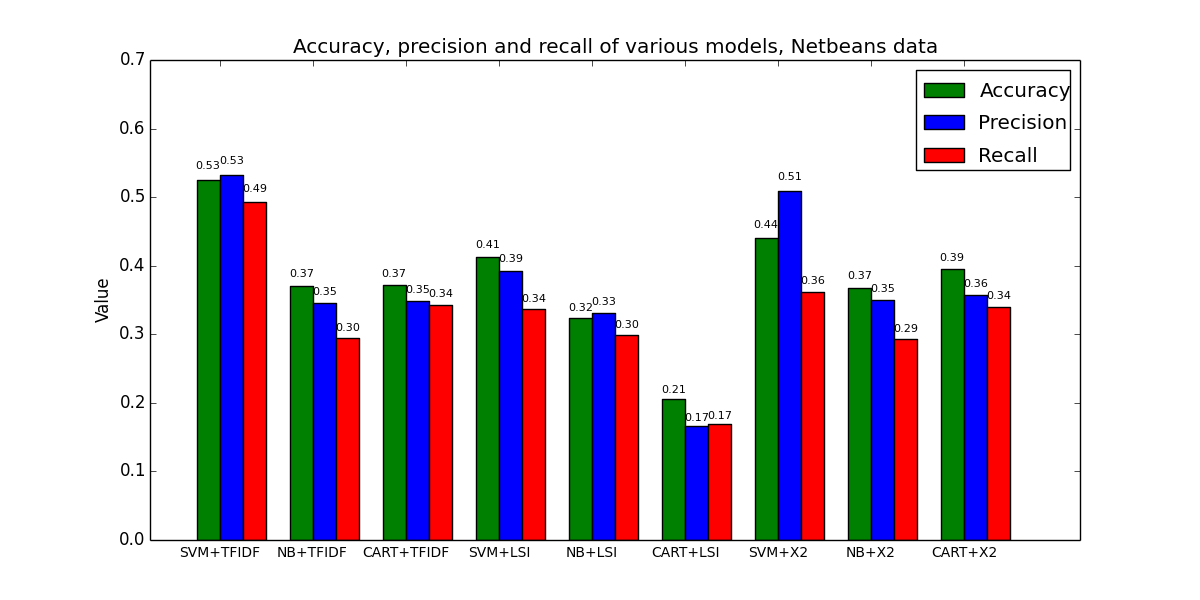
\includegraphics[width=\textwidth,trim=8cm 1cm 8cm 1cm,clip]{./images/comparison_of_models/netbeans.png}
    \caption{Comparison of models on Netbeans data.}
    \label{fig:results.models.netbeans}
\end{figure}

\subsection{Proprietary Data}

In this case, the performance of all models decreased a lot in comparison with the other datasets. However, even in this case, the SVM model with TF-IDF offers the best performance of 37\% accuracy, 32\% precision and 31\% recall. The same model with LSI also shows quite a good performance and quite surprisingly, the Naive Bayes model with LSI performs quite well as far as precision and recall is concerned. Figure~\ref{fig:results.models.proprietary} presents the results in graphical manner.

\begin{figure}[htbp]
    \centering
        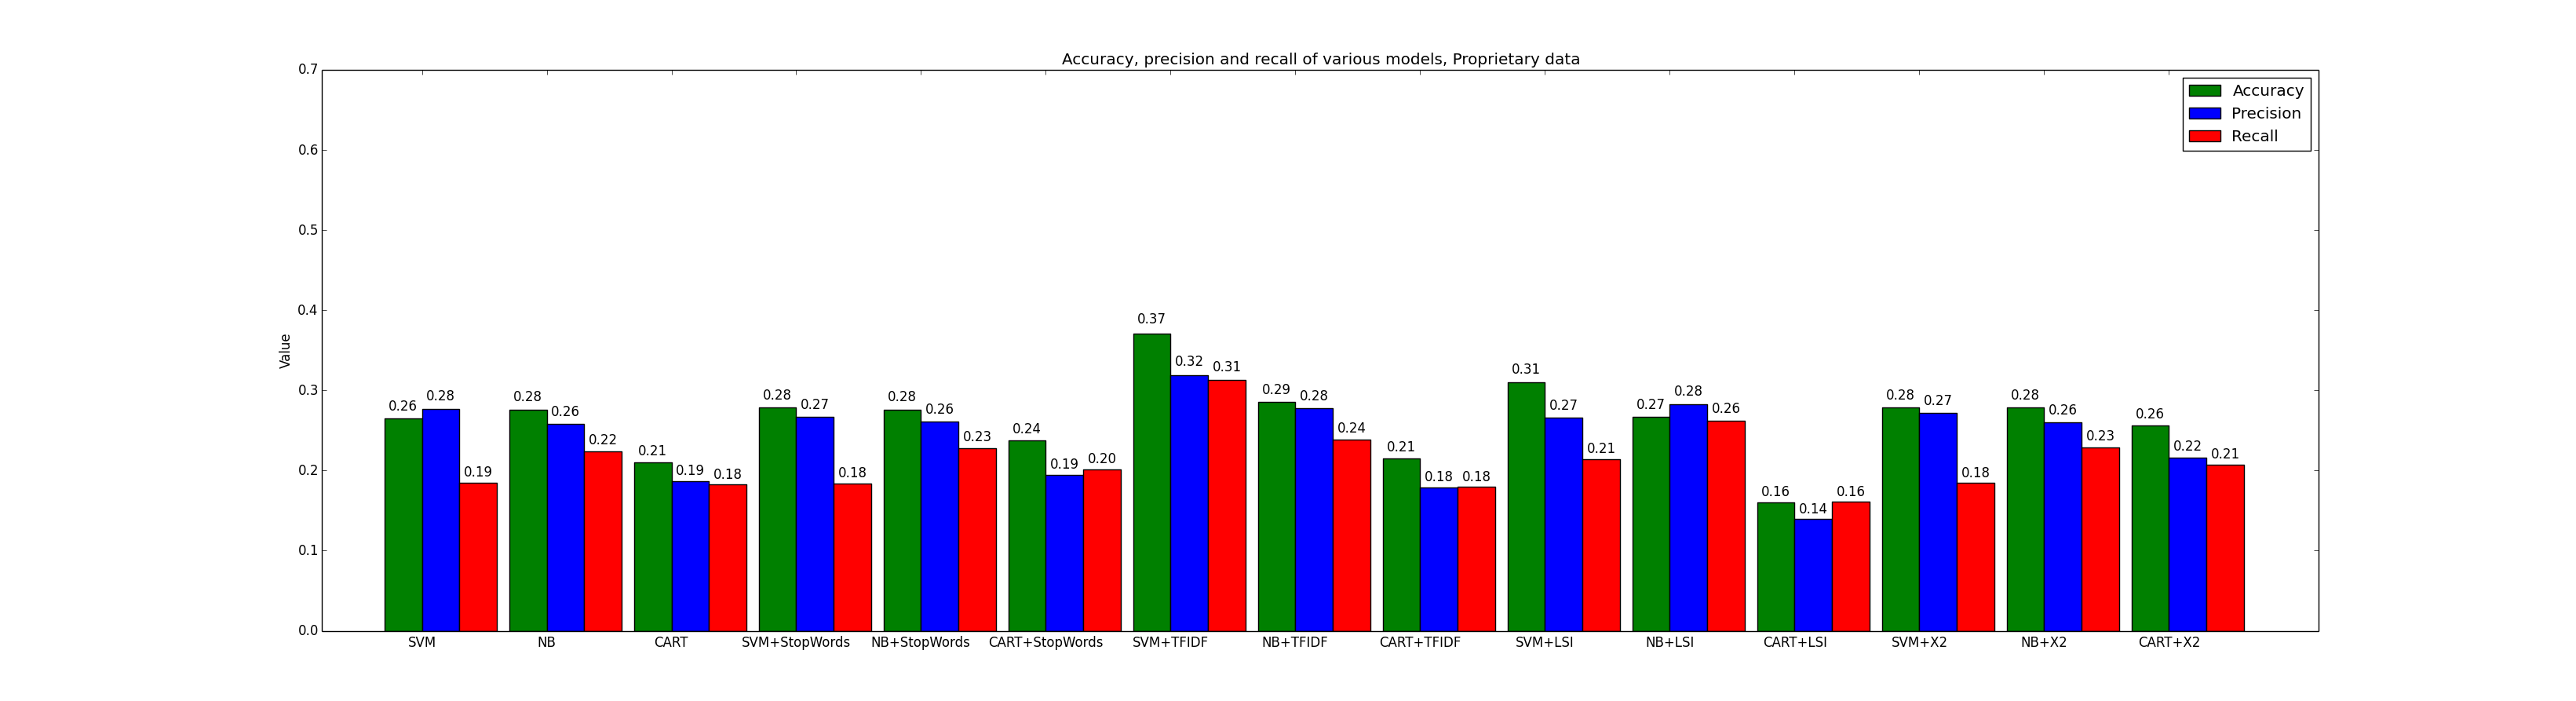
\includegraphics[width=\textwidth,trim=8cm 1cm 8cm 1cm,clip]{./images/comparison_of_models/proprietary.png}
    \caption{Comparison of models on the Proprietary data.}
    \label{fig:results.models.proprietary}
\end{figure}

\subsection{Conclusion}

The comparison shows that SVM with TF-IDF weighing performs best on all datasets. Not only that, it also generalizes very well, because there was no need to readjust the parameters of the model to get the best or nearly the best performance for all datasets. The disadvantage of the model is that it is the most computationally complex one, because SVM is the slowest of the three models, there are a lot of classes and there are a lot of features. This can be at least partially dealt with by using $\chi^2$ feature extraction in conjunction with TF-IDF while sacrificing some of the performance.

\section{Comparison of Datasets}